% =====================================================================
%  Part 3: Implementation results
% =====================================================================
\section{Implementation Results}
\label{sec:results}

Unless stated otherwise, the numbers are test results on the $22{,}594$ complete pairs. They are given as
mean~$\pm$~sample standard deviation over the training seeds $42$, $123$ and $2026$. K0 and T0 are deterministic,
so each has a single value.

\subsection{Training Behaviour}
\label{sec:curves}

\begin{figure}[H]
  \centering
  \begin{subfigure}{0.49\linewidth}
    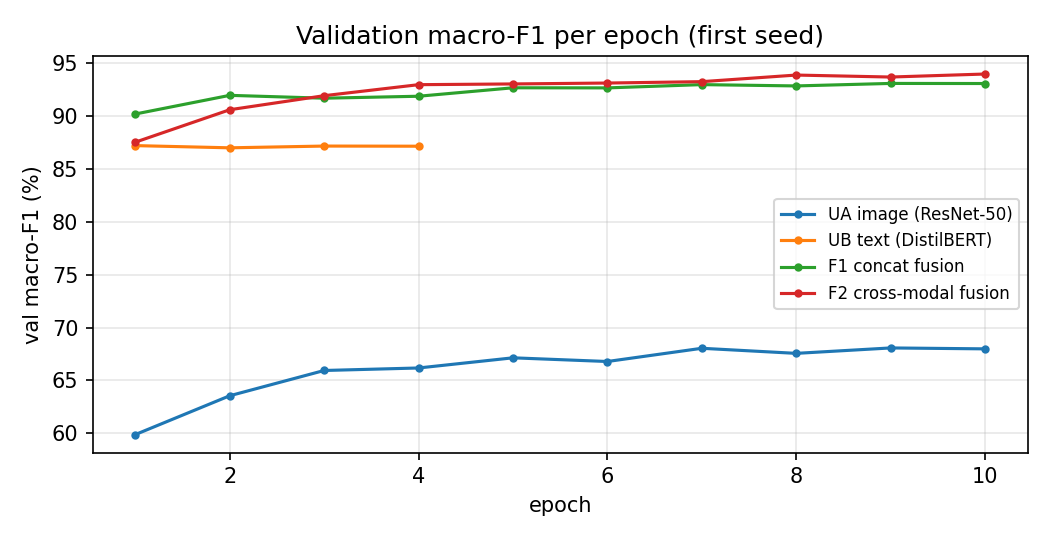
\includegraphics[width=\linewidth]{val_curves.png}
    \caption{Validation macro-F1 per epoch (one seed).}
  \end{subfigure}\hfill
  \begin{subfigure}{0.49\linewidth}
    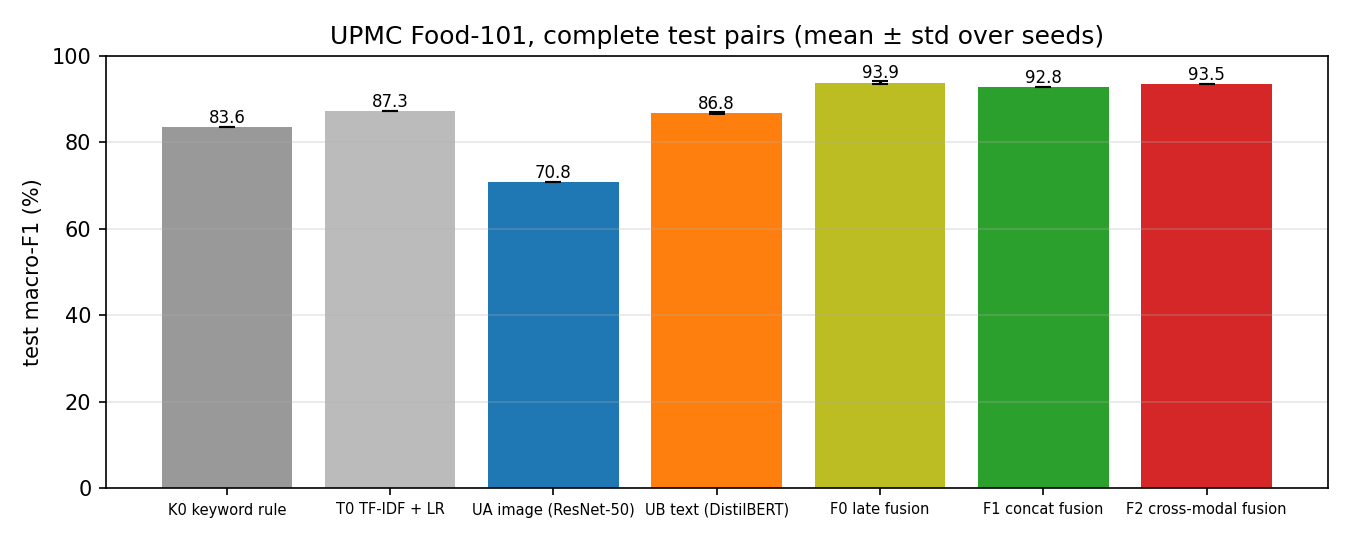
\includegraphics[width=\linewidth]{macro_f1.png}
    \caption{Test macro-F1, mean $\pm$ std.}
  \end{subfigure}
  \caption{Training behaviour and the main result.}
  \label{fig:curves}
\end{figure}

\begin{itemize}
  \item \textbf{UA} improves slowly. Its validation macro-F1 stays around $68\%$; the best epoch is $9$ of $10$.
  \item \textbf{UB} converges after one epoch, at $87\%$ validation macro-F1.
  \item \textbf{F1} starts at $90\%$ after one epoch and fits the training set to $99.7\%$ accuracy.
  \item \textbf{F2}:
        \begin{itemize}
          \item reaches $87.5\%$ after the frozen-encoder epoch, which trains only the $8$\,M new parameters;
          \item passes F1 from epoch~3 and ends at $93.9\%$, with the best epoch between $8$ and $10$;
          \item fits the training set less tightly than F1 ($97.2\%$ against $99.7\%$ accuracy), because the
                auxiliary losses and the modality dropout make the training task harder;
          \item has an auxiliary image head that reaches $68\%$ validation accuracy, as high as the standalone
                image model.
        \end{itemize}
\end{itemize}

\subsection{Unimodal versus Multimodal}
\label{sec:main}

\begin{table}[H]
  \centering\small
  \caption{Main comparison on the complete test pairs. ``Dedup'' removes test items whose image is linked to a
  train image. ``Title unseen'' keeps only the $13{,}701$ test items whose title never occurs in train or validation.}
  \label{tab:main}
  \resizebox{\linewidth}{!}{%
  \begin{tabular}{@{}lcccccc@{}}
    \toprule
    Model & Accuracy & Macro-F1 & Top-5 & ECE & Macro-F1 dedup & Macro-F1 title unseen \\
    \midrule
    K0 keyword rule & $76.95$ & $83.56$ & $77.41$ & $2.97$ & $83.81$ & $82.89$ \\
    T0 TF-IDF + LR  & $87.12$ & $87.26$ & $91.23$ & $2.71$ & $87.36$ & $82.57$ \\
    UA image        & $70.73\pm0.09$ & $70.80\pm0.06$ & $86.51\pm0.16$ & $10.75\pm0.19$ & $67.72\pm0.03$ & $70.59\pm0.12$ \\
    UB text         & $86.42\pm0.91$ & $86.80\pm0.25$ & $90.71\pm0.69$ & $2.84\pm1.46$ & $86.96\pm0.07$ & $82.57\pm0.44$ \\
    \midrule
    F0 late fusion  & $\mathbf{93.93\pm0.23}$ & $\mathbf{93.86\pm0.24}$ & $\mathbf{97.71\pm0.07}$ & $15.98\pm0.78$ & $\mathbf{93.71\pm0.27}$ & $\mathbf{92.03\pm0.32}$ \\
    F1 concat fusion & $92.85\pm0.06$ & $92.80\pm0.06$ & $97.15\pm0.04$ & $4.69\pm0.02$ & $92.80\pm0.07$ & $90.28\pm0.03$ \\
    F2 cross-modal fusion & $93.58\pm0.07$ & $93.53\pm0.07$ & $97.69\pm0.04$ & $\mathbf{2.88\pm0.09}$ & $93.49\pm0.06$ & $91.05\pm0.14$ \\
    \bottomrule
  \end{tabular}}
\end{table}

\begin{table}[H]
  \centering\small
  \caption{Decision rule. $b$ = items that only A classifies correctly, $c$ = items that only B classifies
  correctly (seed 42). A verdict needs both $|\Delta| >$ the larger std and $p<0.05$.}
  \label{tab:decision}
  \begin{tabular}{@{}lrrrrl@{}}
    \toprule
    A vs B & $\Delta$ macro-F1 (pp) & Larger std & $b$ / $c$ & McNemar $p$ & Verdict \\
    \midrule
    UB vs K0 & $+3.24$  & $0.25$ & $2{,}031$ / $128$     & $<10^{-300}$ & UB better \\
    UB vs T0 & $-0.46$  & $0.25$ & $260$ / $655$         & $9\cdot10^{-39}$ & T0 better \\
    UB vs UA & $+16.00$ & $0.25$ & $5{,}503$ / $2{,}219$ & $2\cdot10^{-305}$ & UB better \\
    F0 vs UB & $+7.06$  & $0.25$ & $2{,}068$ / $178$     & $<10^{-300}$ & F0 better \\
    F1 vs UB & $+6.00$  & $0.25$ & $1{,}868$ / $161$     & $<10^{-300}$ & F1 better \\
    F2 vs UB & $+6.73$  & $0.25$ & $2{,}036$ / $168$     & $<10^{-300}$ & F2 better \\
    F1 vs F0 & $-1.06$  & $0.24$ & $426$ / $609$         & $1.5\cdot10^{-8}$ & F0 better \\
    \textbf{F2 vs F1} & $+0.73$ & $0.07$ & $439$ / $278$ & $2.3\cdot10^{-9}$ & \textbf{F2 better} \\
    \textbf{F2 vs F0} & $-0.33$ & $0.24$ & $465$ / $487$ & $0.50$ & \textbf{no decision} \\
    \bottomrule
  \end{tabular}
\end{table}

\begin{enumerate}
  \item \textbf{Text dominates the unimodal results.}
        \begin{itemize}
          \item UB is $16$\,pp above UA, as the proposal hypothesised (E0).
          \item The simple TF-IDF model T0 is even slightly better than UB on the full test set ($+0.46$\,pp,
                significant).
          \item On titles that also occur in training, T0 is more accurate than UB ($93.2$ against $91.7\%$);
                on unseen titles the two are equal ($82.6\%$ macro-F1). The TF-IDF model memorises repeated
                titles a little better. Fine-tuning DistilBERT does not pay off on short titles that mostly name
                the dish.
        \end{itemize}
  \item \textbf{Every fusion clearly beats every unimodal model}, by $6$--$7$\,pp. This holds on the full test set,
        on the dedup subset and on the title-unseen subset.
  \item \textbf{F2 improves over the trained baseline F1} by $0.73$\,pp. The gain is significant, far above the
        seed spread ($0.07$), and also holds on the title-unseen subset ($+0.77$\,pp).
  \item \textbf{F2 does not beat the late fusion F0.} The difference ($-0.33$\,pp) is smaller than F0's seed spread,
        and McNemar finds no difference ($465$ against $487$ discordant items). On complete pairs with informative
        titles, a learned fusion has little to add to averaging two strong unimodal predictions.
        \Cref{sec:e2} shows that this changes when the title carries less direct information.
\end{enumerate}

\subsection{Ablations}
\label{sec:ablation-results}

\subsubsection{E1: auxiliary unimodal losses}

\begin{table}[H]
  \centering\small
  \caption{E1. ``Image head'' and ``text head'' are the accuracies of the auxiliary heads. Without the auxiliary
  losses they are linear probes on the detached features.}
  \label{tab:e1}
  \resizebox{\linewidth}{!}{%
  \begin{tabular}{@{}lcccccc@{}}
    \toprule
    Model & Macro-F1 & Image head & Text head & Acc.\ title removed & Acc.\ image removed & Missing-text set \\
    \midrule
    F2 ($\lambda=0.5$)     & $\mathbf{93.53\pm0.07}$ & $\mathbf{69.7\pm0.4}$ & $\mathbf{87.1\pm0.0}$ & $\mathbf{65.3\pm0.9}$ & $86.7\pm0.2$ & $61.4\pm0.5$ \\
    E1 ($\lambda=0$)       & $93.07\pm0.08$ & $62.3\pm0.1$ & $76.8\pm1.7$ & $58.6\pm0.8$ & $86.3\pm0.1$ & $53.7\pm3.0$ \\
    \bottomrule
  \end{tabular}}
\end{table}

\begin{itemize}
  \item \textbf{Verdict.} The auxiliary losses help: $+0.46$\,pp macro-F1, above the larger std ($0.08$), with
        McNemar $p=3\cdot10^{-7}$.
  \item \textbf{They keep the encoders discriminative.} A linear probe on the image features of E1 reaches only
        $62.3\%$, while the image head of F2 reaches $69.7\%$, close to the standalone UA ($70.7\%$). Without the
        auxiliary losses, joint training lets the image encoder drift away from features that separate the
        classes on their own. This is the ``modality laziness'' seen in F1 in M2. The text features are affected
        even more ($76.8$ against $87.1\%$).
  \item \textbf{Most of the benefit shows when the title is missing}: $+6.7$\,pp with the title removed and $+7.7$\,pp
        on the natural missing-text set. With the image removed, the gain is only $+0.4$\,pp, so the losses
        mainly protect the weaker modality.
\end{itemize}

\subsubsection{E4: modality dropout}

\begin{table}[H]
  \centering\small
  \caption{E4. The natural missing-text set has $121$ items; ``[MISSING]'' feeds the learned missing token instead of the uninformative title.}
  \label{tab:e4}
  \resizebox{\linewidth}{!}{%
  \begin{tabular}{@{}lccccc@{}}
    \toprule
    Model & Macro-F1 & Acc.\ title removed & Acc.\ image removed & Missing-text, as is & Missing-text, [MISSING] \\
    \midrule
    F2 ($p=0.15$) & $93.53\pm0.07$ & $\mathbf{65.3\pm0.9}$ & $86.7\pm0.2$ & $61.4\pm0.5$ & $60.6\pm2.4$ \\
    E4 ($p=0$)    & $93.45\pm0.06$ & $60.6\pm0.4$ & $86.5\pm0.0$ & $58.1\pm1.9$ & $57.9\pm1.4$ \\
    \bottomrule
  \end{tabular}}
\end{table}

\begin{itemize}
  \item \textbf{Verdict on complete pairs: no decision.} The difference is $+0.08$\,pp (McNemar $p=0.54$). The
        modality dropout costs nothing on complete pairs.
  \item \textbf{It helps when the title is missing}: $+4.7$\,pp accuracy with the title removed. It barely matters
        when the image is missing, because the title alone is already almost as good as the full input.
  \item \textbf{Even with both mechanisms, F2 stays below UA without the title} ($65.3$ against $70.7\%$). F0 falls
        back to UA by construction, so it is the most robust model for a missing title (\cref{sec:emod}).
\end{itemize}

\subsubsection{E2: class names masked}
\label{sec:e2}

\begin{table}[H]
  \centering\small
  \caption{E2. Every model is retrained and tested on titles in which every class-name mention is replaced by
  \texttt{[MASK]}. ``Gain over UB'' is the macro-F1 gain of the fusion over the text model of the same seed.}
  \label{tab:e2}
  \resizebox{\linewidth}{!}{%
  \begin{tabular}{@{}lccccc@{}}
    \toprule
    Model & Macro-F1 as is & Macro-F1 masked & $\Delta$ (pp) & Gain over UB, as is & Gain over UB, masked \\
    \midrule
    T0 TF-IDF  & $87.26$ & $47.79$ & $-39.5$ & -- & -- \\
    UB text    & $86.80\pm0.25$ & $43.70\pm0.16$ & $-43.1$ & -- & -- \\
    F0 late    & $\mathbf{93.86\pm0.24}$ & $78.85\pm0.17$ & $-15.0$ & $7.1$ & $35.2$ \\
    F1 concat  & $92.80\pm0.06$ & $80.43\pm0.14$ & $-12.4$ & $6.0$ & $36.7$ \\
    F2 cross-modal & $93.53\pm0.07$ & $\mathbf{81.31\pm0.02}$ & $-12.2$ & $6.7$ & $\mathbf{37.6}$ \\
    \bottomrule
  \end{tabular}}
\end{table}

\begin{itemize}
  \item \textbf{Half of the text signal is the class name.}
        \begin{itemize}
          \item Masking halves the text-only models: UB falls from $86.8$ to $43.7\%$, T0 from $87.3$ to $47.8\%$.
          \item On titles that never named the class, UB scores $39.2\%$ without masking and $39.7\%$ with it, so
                the masking removes the name and nothing else.
          \item What remains in a masked title (ingredients, cooking words, site names, repeated titles) is still
                worth $44\%$, far above chance ($1\%$) but below the image ($70.8\%$). The masked text model is
                $67\%$ accurate on titles seen in train and $28\%$ on unseen ones, so a large part of the
                remainder is memorised page titles.
        \end{itemize}
  \item \textbf{Fusion is much more valuable on masked titles.} The gain over the text model grows from about
        $7$\,pp to $35$--$38$\,pp. All three fusions are also $8$--$11$\,pp above the image model, so the weak
        title still adds information.
  \item \textbf{F2 is the best fusion on masked titles.} It beats F1 by $0.88$\,pp ($p=2\cdot10^{-4}$) and F0 by
        $2.46$\,pp ($p=2\cdot10^{-28}$), with the smallest seed spread ($0.02$). When neither modality is decisive,
        token-level cross-attention combines the partial evidence better than averaging two probability vectors.
        This reverses the F0--F1 ranking of the unmasked titles.
\end{itemize}

\subsection{Modality Removal (E-mod) and Missing Modality}
\label{sec:emod}

\begin{figure}[H]
  \centering
  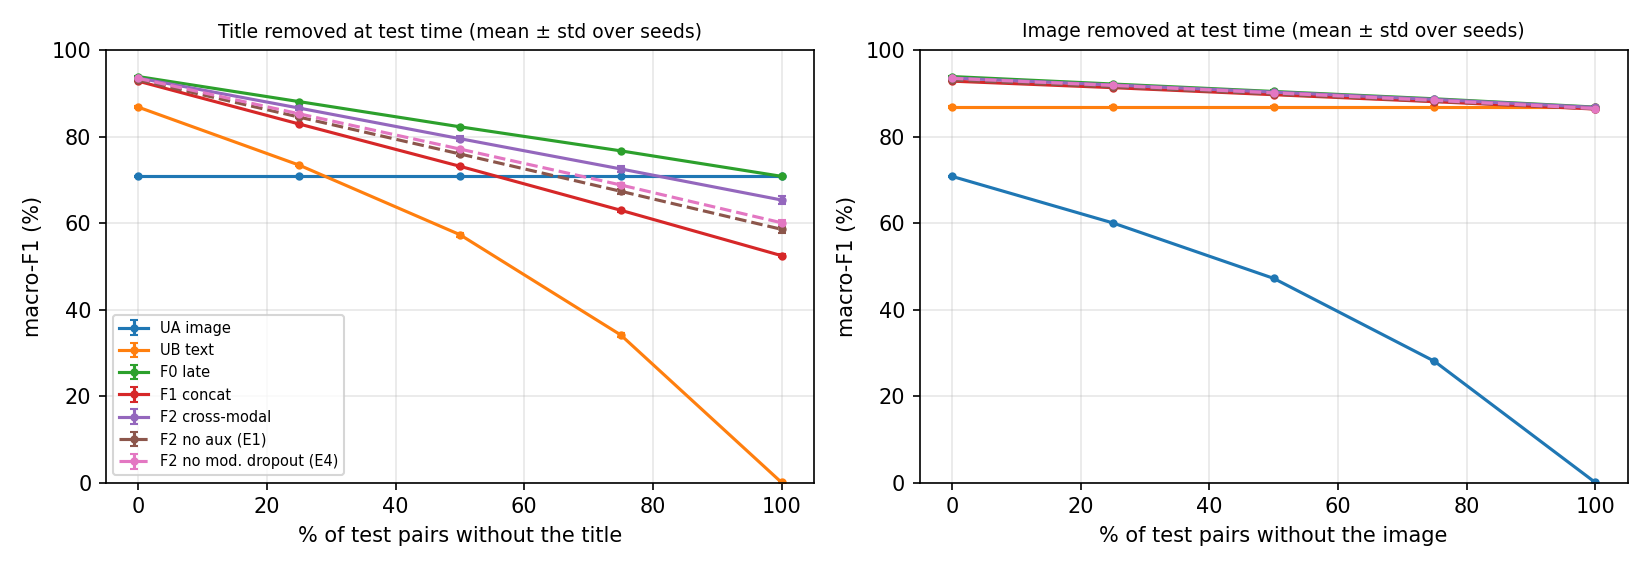
\includegraphics[width=\linewidth]{removal_curves.png}
  \caption{Macro-F1 when the title (left) or the image (right) is removed from a random fraction of the complete
  test pairs, without retraining. Removed items use each model's fallback (\cref{sec:ablations}).}
  \label{fig:removal}
\end{figure}

\begin{itemize}
  \item \textbf{Linear curves.} The removed items are drawn at random, so each curve is a linear mix of the
        full-input and the single-modality accuracy. The end points carry all the information; the slope shows how
        much each model depends on a modality.
  \item \textbf{Removing the image costs every fusion about $7$\,pp.} All fusions end at the text model's level
        ($86.3$--$86.8\%$).
  \item \textbf{Removing the title separates the models}, as shown by macro-F1 with $100\%$ of the titles removed:
        \begin{itemize}
          \item F0: $70.8\%$, because it falls back to UA;
          \item F2: $65.3\%$;
          \item F2 without modality dropout (E4): $60.1\%$;
          \item F2 without auxiliary losses (E1): $58.5\%$;
          \item F1: $52.5\%$.
        \end{itemize}
        F2's two mechanisms close more than half of F1's gap to the image model, but not all of it.
  \item \textbf{Natural missing-text set} ($121$ items with an invalid title), accuracy:
        \begin{itemize}
          \item UA: $65.6\%$; UB: $6.3\%$;
          \item F0: $68.9\%$ with the title as is;
          \item F2: $61.4\%$ with the title as is, $60.6\%$ with its \texttt{[MISSING]} token;
          \item F1: $51.8\%$. This value comes from the M2 evaluation, which zero-filled the text in both
                variants.
        \end{itemize}
\end{itemize}

\subsection{Support and Conflict Analysis (three seeds)}
\label{sec:support}

\begin{table}[H]
  \centering\small
  \caption{Fusion accuracy per group, mean over seeds. The groups come from UA and UB of the same seed.
  ``Follows image'' = share of items where the fused prediction equals UA's.}
  \label{tab:support}
  \resizebox{\linewidth}{!}{%
  \begin{tabular}{@{}lrrrrrrrr@{}}
    \toprule
    Group & Items & Share & F0 & F1 & F2 & E1 & E4 & F2 follows image \\
    \midrule
    Support (both right)          & $13{,}938$ & $61.7\%$ & $100.0$ & $99.8$ & $99.8$ & $99.8$ & $99.8$ & $99.8\%$ \\
    Conflict-I (only image right) & $2{,}043$  & $9.0\%$  & $\mathbf{90.6\pm4.5}$ & $69.0\pm2.7$ & $75.3\pm2.0$ & $70.9\pm1.3$ & $74.7\pm1.6$ & $75.3\%$ \\
    Conflict-T (only text right)  & $5{,}588$  & $24.7\%$ & $97.1\pm0.9$ & $97.7\pm0.1$ & $97.7\pm0.2$ & $\mathbf{97.9\pm0.2}$ & $97.8\pm0.2$ & $1.2\%$ \\
    Both wrong, same prediction   & $150$      & $0.7\%$  & $0.0$ & $10.7$ & $10.6$ & $10.7$ & $10.0$ & $84.3\%$ \\
    Both wrong, different         & $875$      & $3.9\%$  & $0.7$ & $21.3$ & $\mathbf{24.0}$ & $22.6$ & $23.2$ & $18.9\%$ \\
    \bottomrule
  \end{tabular}}
\end{table}

\begin{figure}[H]
  \centering
  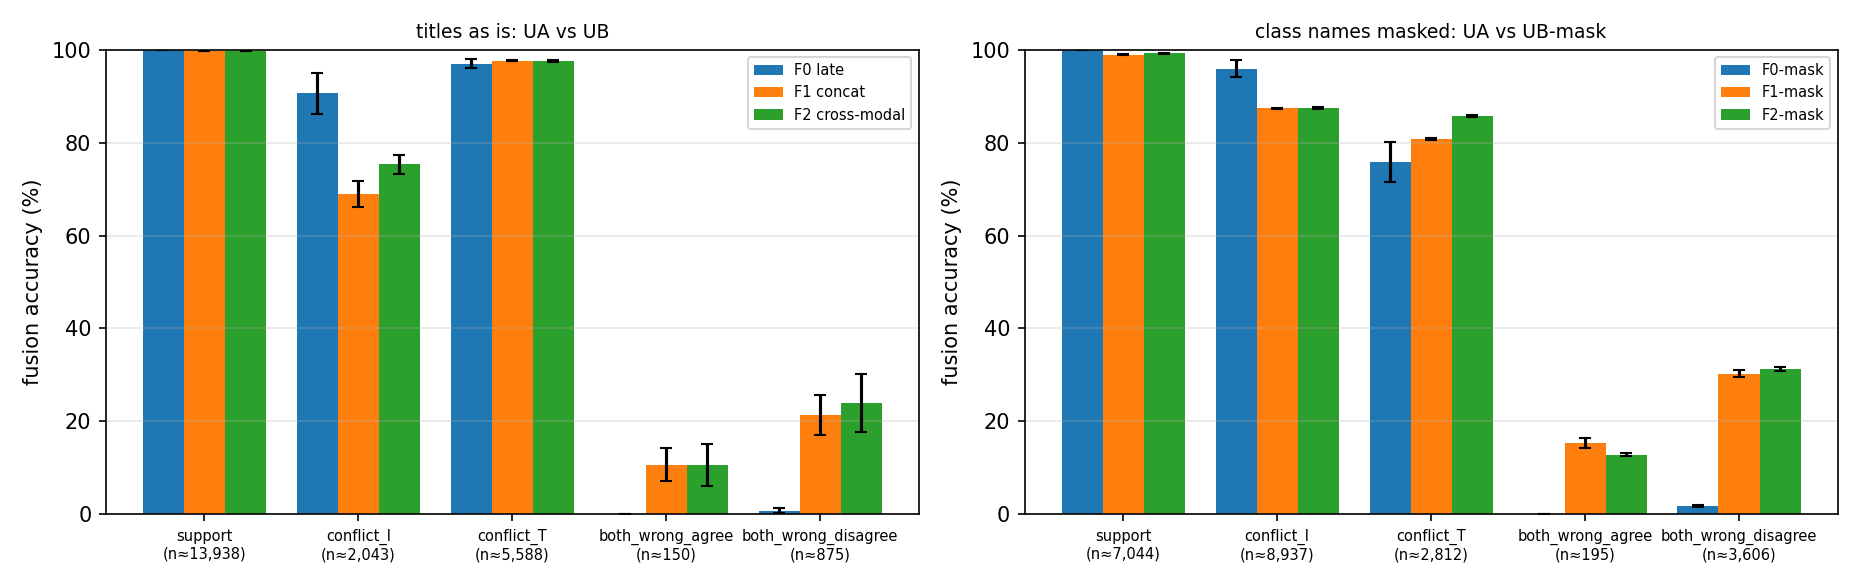
\includegraphics[width=\linewidth]{support_conflict_seeds.png}
  \caption{Fusion accuracy per group over three seeds, with titles as is (left) and with class names masked (right).}
  \label{fig:support}
\end{figure}

\begin{itemize}
  \item \textbf{Stable over seeds.} The M2 conclusions (seed 42 only) hold over three seeds:
        \begin{itemize}
          \item support items are solved by every model;
          \item the fusion gain comes from the conflict groups;
          \item a misleading title (Conflict-I) is the weak spot of the trained fusions.
        \end{itemize}
  \item \textbf{Conflict-I.} F2 recovers $75.3\%$ of these items, against $69.0\%$ for F1. This is $+6.3$\,pp, and
        E1 shows that the auxiliary losses account for most of it ($70.9\%$ without them). F0 still recovers the
        most ($90.6\%$). Its averaging lets a confident image prediction outvote an uncertain title, while F2 still
        follows the title in a quarter of these items.
  \item \textbf{Both wrong.} The trained fusions are the only models that solve some items on which both unimodal
        models fail. F2 solves $24\%$ of the items where UA and UB disagree. A late fusion can only choose between
        the two unimodal predictions, so it cannot do this.
  \item \textbf{With masked titles (right panel), the balance shifts.} Conflict-I becomes the largest group
        ($40\%$). F2-mask is the best model on Conflict-T ($85.7\%$ against $75.9\%$ for F0-mask) and on the
        items where both unimodal models are wrong and disagree ($31.2\%$). This is where its overall advantage on masked titles comes from.
\end{itemize}

\subsection{Qualitative Analysis: Grad-CAM and \texttt{[FUS]} Attention}
\label{sec:qualitative}

\begin{figure}[H]
  \centering
  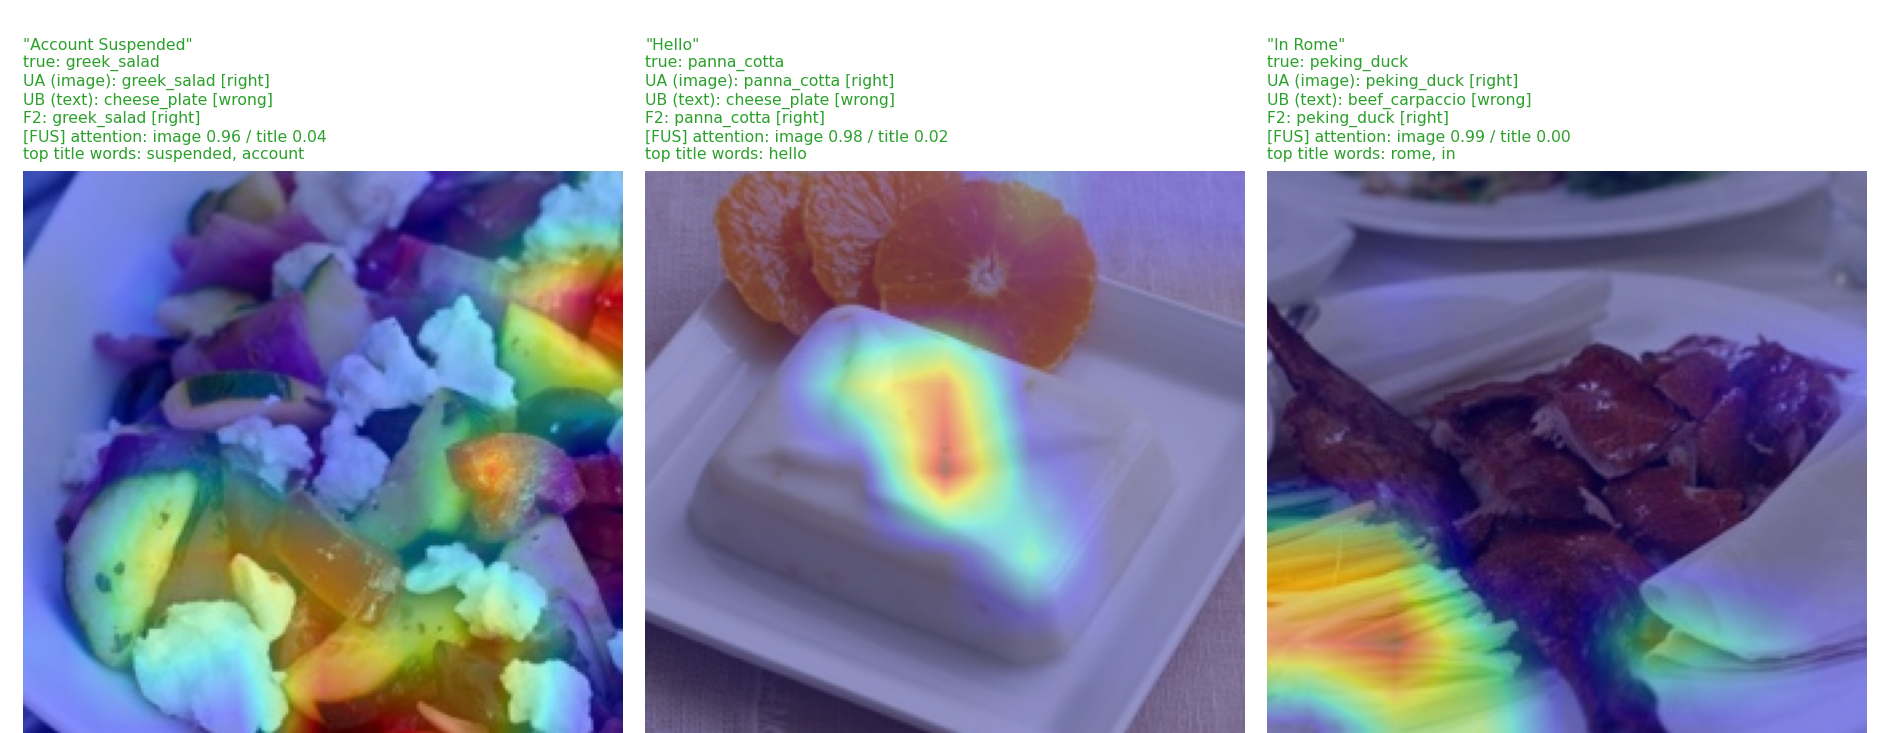
\includegraphics[width=\linewidth]{qual_conflict_I.png}
  \caption{Conflict-I examples (seed 42): the image model is right and the text model is wrong. Grad-CAM of F2's
  image encoder for F2's predicted class; title in green if F2 is right.}
  \label{fig:qual-i}
\end{figure}

\begin{figure}[H]
  \centering
  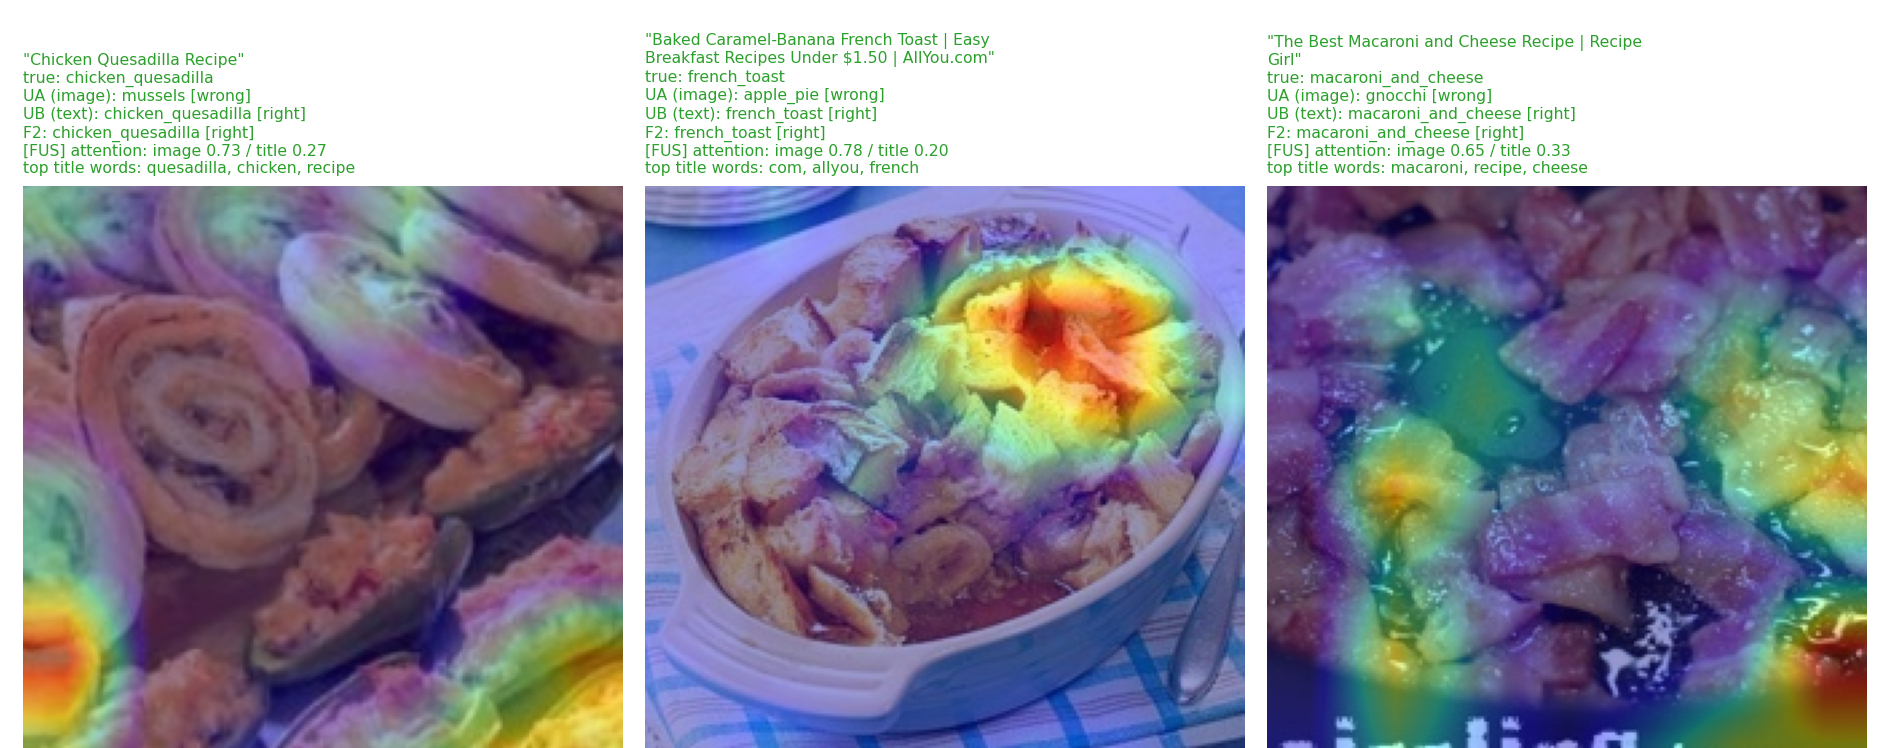
\includegraphics[width=\linewidth]{qual_conflict_T.png}
  \caption{Conflict-T examples (seed 42): the text model is right and the image model is wrong.}
  \label{fig:qual-t}
\end{figure}

\begin{table}[H]
  \centering\small
  \caption{Mean share of the \texttt{[FUS]} attention on the image tokens (last fusion layer, seed 42). The rest goes
  to the title tokens and to \texttt{[FUS]} itself.}
  \label{tab:attention}
  \begin{tabular}{@{}lccccc@{}}
    \toprule
    Model & All & Support & Conflict-I & Conflict-T & Both wrong \\
    \midrule
    F2       & $0.805$ & $0.792$ & $\mathbf{0.909}$ & $0.778$ & $0.891$ \\
    E1 (no aux.) & $0.756$ & $0.745$ & $0.873$ & $0.720$ & $0.847$ \\
    E4 (no mod.\ dropout) & $0.883$ & $0.883$ & $0.930$ & $0.858$ & $0.917$ \\
    F2-mask  & $0.922$ & $0.928$ & $0.927$ & $0.907$ & $0.912$ \\
    \bottomrule
  \end{tabular}
\end{table}

\begin{itemize}
  \item \textbf{F2 shifts its attention item by item.} On Conflict-I items, whose titles are uninformative, $91\%$
        of the \texttt{[FUS]} attention goes to the image. On Conflict-T items it is $78\%$. In
        \cref{fig:qual-i}, titles such as ``Account Suspended'', ``Hello'' or ``In Rome'' get $0$--$4\%$ of the
        attention, and F2 classifies from the image. In \cref{fig:qual-t}, the title words that name the dish
        (``quesadilla'', ``macaroni'', ``cheese'') receive the most attention.
  \item \textbf{The shares should be compared between groups, not read as absolute values.} The image has $49$
        tokens against about $15$ for a title, so a uniform attention would already give about $0.75$ to the
        image. E1 attends less to the image ($0.756$), which fits its weaker image branch. F2-mask attends more
        ($0.922$), which fits a less informative title.
  \item \textbf{Grad-CAM} usually highlights the food rather than the plate or the background. Two kinds of failure
        recur:
        \begin{itemize}
          \item the map spreads over a mix of dishes, for example the starter platter labelled
                \cls{chicken\_quesadilla} in \cref{fig:qual-t};
          \item the map lands on text overlaid on the image (``sizzling bacon'').
        \end{itemize}
        Both are cases where the image alone is misleading and the title has to decide.
\end{itemize}

\subsection{Error Taxonomy of the Conflict Cases}
\label{sec:taxonomy}

\begin{table}[H]
  \centering\small
  \caption{Main cause of the failing unimodal model in $100$ random conflict items (seed 42), with Wilson 95\%
  intervals~\cite{wilson1927}. The last three columns give the accuracy of the fusion models on the same items.}
  \label{tab:taxonomy}
  \resizebox{\linewidth}{!}{%
  \begin{tabular}{@{}llrrrrr@{}}
    \toprule
    Group (failing model) & Cause & Items & Share (95\% CI) & F0 & F1 & F2 \\
    \midrule
    Conflict-I (text wrong)  & title generic (no dish information)   & $42$ & $84\%$ ($71$--$92$) & $100$ & $74$ & $93$ \\
                             & title names another dish             & $8$  & $16\%$ ($8$--$29$)  & $50$ & $38$ & $50$ \\
    \midrule
    Conflict-T (image wrong) & visually similar to another dish     & $34$ & $68\%$ ($54$--$79$) & $94$ & $94$ & $100$ \\
                             & image unrelated (no dish, collage, \dots) & $13$ & $26\%$ ($16$--$40$) & $100$ & $100$ & $100$ \\
                             & wrong label                          & $2$  & $4\%$ ($1$--$13$)   & $100$ & $100$ & $100$ \\
                             & other                                & $1$  & $2\%$ ($0$--$10$)   & $100$ & $100$ & $100$ \\
    \bottomrule
  \end{tabular}}
\end{table}

\begin{itemize}
  \item \textbf{The text model fails mostly on generic titles}, such as a site name, ``Hello'' or a drinks brand,
        not on wrong ones. F0 and F2 fix almost all of these items; F1 fixes only three quarters.
  \item \textbf{The hard case is a title that names another dish}, for example ``French Bread Pizza'' for a
        \cls{pizza} image, which UB reads as \cls{garlic\_bread}. Every fusion solves only about half of these
        items, because the title actively points to a wrong class instead of carrying no information.
  \item \textbf{The image model fails mostly on dishes that look alike} or on unusual plating, such as a beef
        tartare tower topped with caviar that it reads as cupcakes. Here F2 is the only model that solves every
        reviewed item.
  \item \textbf{Wrong labels are rare} ($2$ of $100$), in line with the $0.5\%$ of the M2 pair audit.
  \item \textbf{Repeated titles.} In $28\%$ of the reviewed items, the title also occurs in train or
        validation. Some correct text predictions are memorised: the title ``- quoteko.com'' occurs $80$ times in
        train and validation, $77$ of them as \cls{breakfast\_burrito}, so UB predicts that class with $98\%$
        confidence for an image of baked oatmeal. Other correct text predictions are lucky guesses with a
        confidence of a few percent.
  \item \textbf{Limitations.} The sample is small: the ``another dish'' group has $8$ items. Each item was labelled
        by one reviewer, so there is no inter-rater agreement.
\end{itemize}

\subsection{Leakage Checks}
\label{sec:leakage}

\begin{table}[H]
  \centering\small
  \caption{Accuracy on test titles that do or do not occur in train/validation, and macro-F1 on unseen titles.}
  \label{tab:leakage}
  \begin{tabular}{@{}lrrr@{}}
    \toprule
    Model & Acc.\ title seen ($8{,}893$) & Acc.\ title unseen ($13{,}701$) & Macro-F1 unseen \\
    \midrule
    UA image  & $70.18$ & $71.09$ & $70.59$ \\
    UB text   & $91.71$ & $82.99$ & $82.57$ \\
    T0 TF-IDF & $93.24$ & $83.14$ & $82.57$ \\
    F0 late   & $95.88$ & $92.67$ & $\mathbf{92.03}$ \\
    F1 concat & $95.76$ & $90.96$ & $90.28$ \\
    F2 cross-modal & $96.44$ & $91.73$ & $91.05$ \\
    \bottomrule
  \end{tabular}
\end{table}

\begin{itemize}
  \item \textbf{Repeated titles inflate every text-using model by $3$--$10$\,pp.} The image model, which never sees
        the title, is a control: it is as accurate on both subsets.
  \item \textbf{The ranking and every decision of \cref{tab:decision} hold on the title-unseen subset.} F2 is
        $0.77$\,pp above F1 and $1.0$\,pp below F0 there.
  \item \textbf{Image duplicates} inflate only the image model ($-3.1$\,pp on the dedup subset). Every fusion
        loses at most $0.2$\,pp there.
\end{itemize}

\subsection{Calibration}
\label{sec:calibration}

\begin{table}[H]
  \centering\small
  \caption{Test ECE (\%) before and after temperature scaling; $T$ is fitted on validation.}
  \label{tab:calibration}
  \resizebox{\linewidth}{!}{%
  \begin{tabular}{@{}lrrr@{\hspace{2em}}lrrr@{}}
    \toprule
    Model & $T$ & Before & After & Model & $T$ & Before & After \\
    \midrule
    UA & $1.62$ & $10.75$ & $4.22$ & F2 & $1.40$ & $\mathbf{2.88}$ & $\mathbf{0.45}$ \\
    UB & $1.30$ & $2.84$ & $1.01$  & E1 & $1.39$ & $3.02$ & $0.59$ \\
    F0 & $0.61$ & $15.98$ & $6.46$ & E4 & $1.59$ & $3.57$ & $0.56$ \\
    F1 & $1.91$ & $4.69$ & $0.90$  & F2-mask & $1.50$ & $8.43$ & $0.83$ \\
    \bottomrule
  \end{tabular}}
\end{table}

\begin{itemize}
  \item \textbf{F2 is the best-calibrated model}, both before and after temperature scaling.
  \item \textbf{One temperature brings every trained model to about $1\%$ ECE or less}, except UA ($4.2\%$).
  \item \textbf{F0 stays badly calibrated}, because a single temperature cannot fix it. Its averaged probabilities
        are under-confident ($T<1$ sharpens them). The confidence of F0 is therefore the least usable, even
        though its accuracy is the highest.
\end{itemize}

\subsection{Compute Cost}
\label{sec:cost}

\begin{table}[H]
  \centering\small
  \caption{Compute cost on the RTX A6000 (shared). Inference uses bf16, $224$\,px images and titles trimmed per
  batch. T0 runs on the CPU.}
  \label{tab:cost}
  \resizebox{\linewidth}{!}{%
  \begin{tabular}{@{}lrrrrrr@{}}
    \toprule
    Model & Params & GMACs/item & Train time/run & Train items/s & Inference items/s & Latency \\
     & & & & & (batch 128) & (batch 1) \\
    \midrule
    T0 & $13.6$\,M & -- & $4.4$\,min (CPU) & -- & -- & -- \\
    UA & $23.71$\,M & $4.09$ & $14.4$\,min & $728$   & $2{,}793$  & $4.7$\,ms \\
    UB & $66.44$\,M & $0.64$ & $2.0$\,min  & $2{,}420$ & $17{,}105$ & $2.7$\,ms \\
    F0 & $90.15$\,M & $4.73$ & $16.4$\,min (UA + UB) & -- & $\approx 2{,}400$ & $\approx 7.4$\,ms \\
    F1 & $91.89$\,M & $4.73$ & $18.4$\,min & $568$   & $2{,}385$  & $7.7$\,ms \\
    F2 & $97.98$\,M & $5.06$ & $18.6$\,min & $526$   & $2{,}220$  & $8.5$\,ms \\
    \bottomrule
  \end{tabular}}
\end{table}

\begin{itemize}
  \item \textbf{F2's improvement is cheap.} It costs $7\%$ more computation and $1$--$2\%$ more training time than F1.
        The frozen first epoch is fast ($45$\,s against $120$\,s).
  \item \textbf{F0 has the same cost as running UA and UB}: its inference figures are the sum of the two models.
        It needs no extra training.
  \item \textbf{Total compute.}
        \begin{itemize}
          \item M2: $9$ runs in $2.0$ GPU-hours.
          \item M3: $18$ runs ($4.75$ hours of training) plus evaluation, removal predictions and Grad-CAM, in
                about $5.7$ GPU-hours.
        \end{itemize}
        The whole assignment therefore used about $7.7$ GPU-hours, within the $6$--$8$ hours re-budgeted in M2.
\end{itemize}

\subsection{Limitations}
\label{sec:limits}

\begin{itemize}
  \item \textbf{Fixed test list.} The official test list cannot be regrouped: $14.5\%$ of its items have a train
        image duplicate and $39\%$ share a title with train. We report leakage-controlled views instead.
  \item \textbf{Validation shares titles with train.} The validation set is grouped by image clusters only. Model
        selection is affected in the same way for all models.
  \item \textbf{Titles only.} The results are not directly comparable with full-text results in the literature.
  \item \textbf{Small review sample.} The error taxonomy rests on $100$ items with one reviewer each.
  \item \textbf{One F2 configuration.} There was no search over F2's depth, $\lambda$ or $p$; the proposal fixed
        them. E3 (frozen encoders) was dropped for time.
  \item \textbf{Shared GPU.} The measured throughput depends on the other jobs that were running on the same GPU.
\end{itemize}
